\subsection{Unscented Kalman Filter on Manifolds}
\subsubsection{Concept and Motivation}
Up to this point, all Kalman Filter variants, including the EKF and ESKF, approximate nonlinear systems locally through 1st order linearization. Although effective for mildly nonlinear dynamics, these methods rely on Jacobians, which introduce errors when the system exhibits strong nonlinearity or discontinuous dynamics. An alternative approach to local linearization is sampling based nonlinear approximation. A well known technique of this class is the \textit{``Unscented Transform (UT)''}, which represents a Gaussian distribution using a small, deterministically chosen set of sample points (called sigma points) and then propagates them through the nonlinear function to capture the transformed mean and covariance up to the third order for Gaussian inputs \cite{ukf}.
\begin{figure}[H]
    \centering
    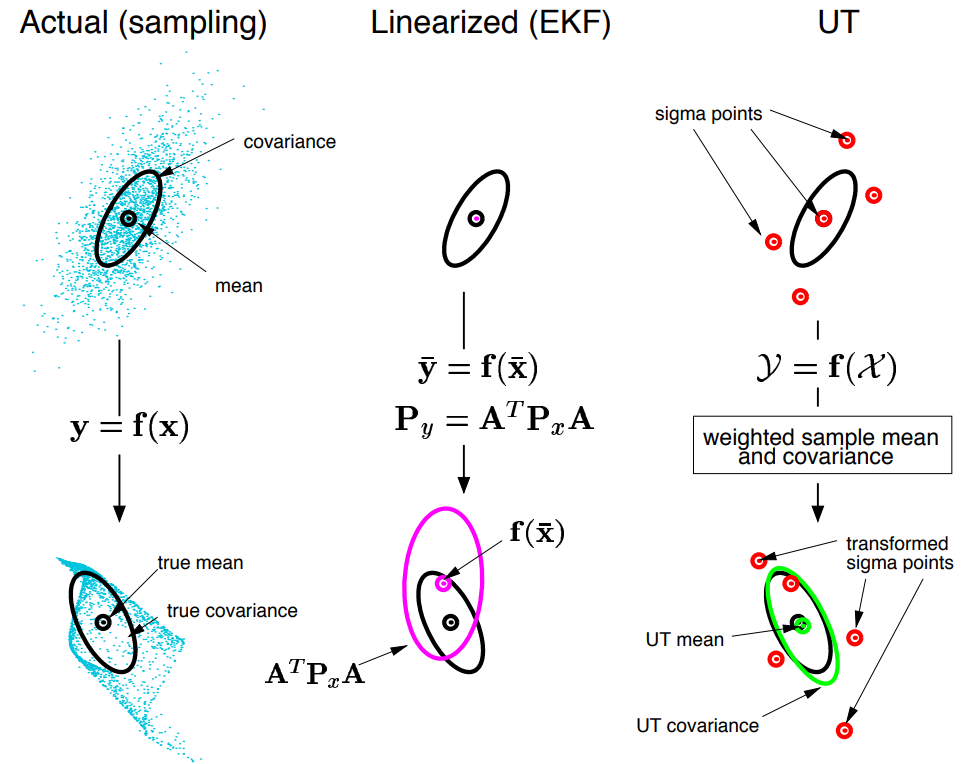
\includegraphics[width=0.7\linewidth]{Pictures/State_Estimation/Unscented_Kalman_Filter_on_Manifolds/Unscented_Transform.png}
    \caption{Comparison of different methods for nonlinear mean and covariance propagation. The figure contrasts (a) direct sampling of the true nonlinear distribution, (b) linearization using the Extended Kalman Filter (EKF), and (c) the Unscented Transform (UT), which captures the mean and covariance more accurately without linearization. Image taken from Unscented Kalman Filter paper.\textsuperscript{\cite{ukf}}}
    \label{fig:state-estimation-uncented-transform}
\end{figure}



\subsubsection{Unscented Kalman Filter}
The Unscented Transform is defined by generating a set of $2L + 1$ sigma points from the prior mean $\mathbf{x}$ and covariance $P$, where $L$ denotes the dimensionality of the state vector. Each sigma point represents a deterministic sample capturing the local mean and covariance structure of the state distribution, ensuring accurate nonlinear propagation up to the second order for any nonlinearity.
$$
\begin{aligned}
    \chi_0 &= \mathbf{x} \\
    \chi_i &= \mathbf{x} + (\sqrt{(L + \lambda)P_i})              && i = 1, \ldots, L \\
    \chi_i &= \mathbf{x} - (\sqrt{(L + \lambda)P_{i - L} })       && i = L+1, \ldots, 2L
\end{aligned}
$$
$$
    \lambda = \alpha^2 (L + \kappa) - L
$$
where $\lambda$ is a scaling parameter controlling the spread of the sigma points. Each sigma point is assigned associated weights $W_i^m$ and $W_i^c$ for mean and covariance reconstruction. These weights ensure that both the central and surrounding sigma points contribute correctly to the nonlinear mean and covariance propagation according to their statistical significance. The weights are defined as
$$
\begin{aligned}
    W_0^m &= \frac{\lambda}{L + \lambda} \\
    W_0^c &= \frac{\lambda}{L + \lambda} + (1 - \alpha^2 + \beta) \\
    W_i^m &= W_i^c = \frac{1}{2(L + \lambda)}                           && i = 1, \ldots, 2L
\end{aligned}
$$
The parameters $\alpha$, $\beta$, and $\kappa$ govern the spread, scaling, and higher order accuracy of the sigma point distribution. According to the original Unscented Kalman Filter formulation by Julier and Uhlmann \cite{ukf}, these parameters should be tuned to balance numerical stability and approximation accuracy. The parameter $\alpha$ determines the overall spread of the sigma points around the mean, it is typically chosen as a small positive value ($10^{-3} \leq \alpha \leq 1$), with smaller values resulting in sigma points closer to the mean and larger values increasing the nonlinear coverage at the cost of potential numerical instability. The parameter $\kappa$ acts as a secondary scaling term that adjusts the effective spread of the sigma points; it is often set to $0$ for simplicity or $3 - L$ to guarantee positive semi definiteness of the covariance. The parameter $\beta$ encodes prior knowledge of the underlying distribution, for Gaussian distributions, $\beta = 2$ is recommended, as it ensures optimal 2nd order accuracy in the covariance reconstruction. 
\\ \\  
Together, these parameters define how the sigma points are positioned and weighted to best approximate the true nonlinear mean and covariance transformation while maintaining numerical stability across a wide range of system non-linearities. 
\\ \\  
Using these sigma points and weights, the propagated mean and covariance are computed as
$$
\begin{aligned}
    \hat{\mathbf{x}}^- &= \sum_{i=0}^{2L} W_i^m f_d(\chi_i, \mathbf{u}) \\
    P^- &= \sum_{i=0}^{2L} W_i^c [f_d(\chi_i, \mathbf{u}) - \hat{\mathbf{x}}][f_d(\chi_i, \mathbf{u}) - \hat{\mathbf{x}}]^\top
\end{aligned}
$$
This process effectively replaces linearization and analytical Jacobian computation with a deterministic sampling of the nonlinear function. A similar procedure is applied during the measurement update step, where the sigma points are propagated through the nonlinear measurement model $h(\mathbf{x})$ to compute the predicted observation mean and covariance.
\\ \\
During the measurement update step, each predicted sigma point $\chi_i^-$ is passed through the nonlinear measurement model $h(\mathbf{x})$ (for example, the GNSS measurement model in Equation \ref{eq:aiding-measurement-model}) to get predicted measurement samples:
$$
    \mathcal{Z}_i = h(\chi_i^-)
$$
The predicted measurement sample mean is computed as
$$
    \hat{\mathbf{z}} = \sum_{i=0}^{2L} W_i^m \, \mathcal{Z}_i
$$
The corresponding innovation covariance and cross covariance are then obtained as
$$
    S = \sum_{i=0}^{2L} W_i^c \, (\mathcal{Z}_i - \hat{\mathbf{z}})(\mathcal{Z}_i - \hat{\mathbf{z}})^\top + R
$$
$$
    P_{xz} = \sum_{i=0}^{2L} W_i^c \, (\chi_i^- - \hat{\mathbf{x}}^-)(\mathcal{Z}_i - \hat{\mathbf{z}})^\top,
$$
where $R$ is the measurement noise covariance matrix.  
\\ \\
The Kalman gain is then computed as
$$
    K = P_{xz} S^{-1}.
$$
The state and covariance are updated according to
$$
    \hat{\mathbf{x}} = \hat{\mathbf{x}}^- + K(\mathbf{z} - \hat{\mathbf{z}}),
$$
$$
    P = P^- - K S K^\top.
$$
Finally, the quaternion component of the state is normalized to maintain unit length and ensure a valid rotation representation:
$$
    \mathbf{q} \leftarrow \frac{\mathbf{q}}{\|\mathbf{q}\|}.
$$
This completes the classical UKF update stage, where non-linearities are handled through sigma point sampling rather than analytic Jacobian linearization.



\subsubsection{Manifold Operators}
The classical UKF assumes that all system states evolve in Euclidean space $\mathbb{R}^n$. However, many real world systems and motion models, such as INS motion model \ref{eq:kinematics-motion-model}, include quantities that lie on nonlinear manifolds. A common example is the attitude represented by unit quaternions $\mathbf{q} \in \mathbb{S}^3$, which form a curved space where addition and averaging are not globally valid operations. Applying the standard UKF directly to such states can lead to inconsistencies, since linear updates may move the estimate off the manifolds surface.  
\\ \\
The \textit{``Unscented Kalman Filter on Manifolds (UKF-M)''} \cite{ukf_manifold} extends the standard UKF by performing all statistical operations within the tangent space of the manifold. The Unscented Transform is carried out locally in this Euclidean tangent space, and the resulting sigma points are mapped back to the manifold using the exponential and logarithmic maps introduced in Equations \ref{eq:lie-groups-and-manifold-exponential} and \ref{eq:lie-groups-and-manifold-logarithmic}. This approach ensures that all propagated and updated states remain geometrically consistent.  
\\ \\
\begin{figure}[H]
    \centering
    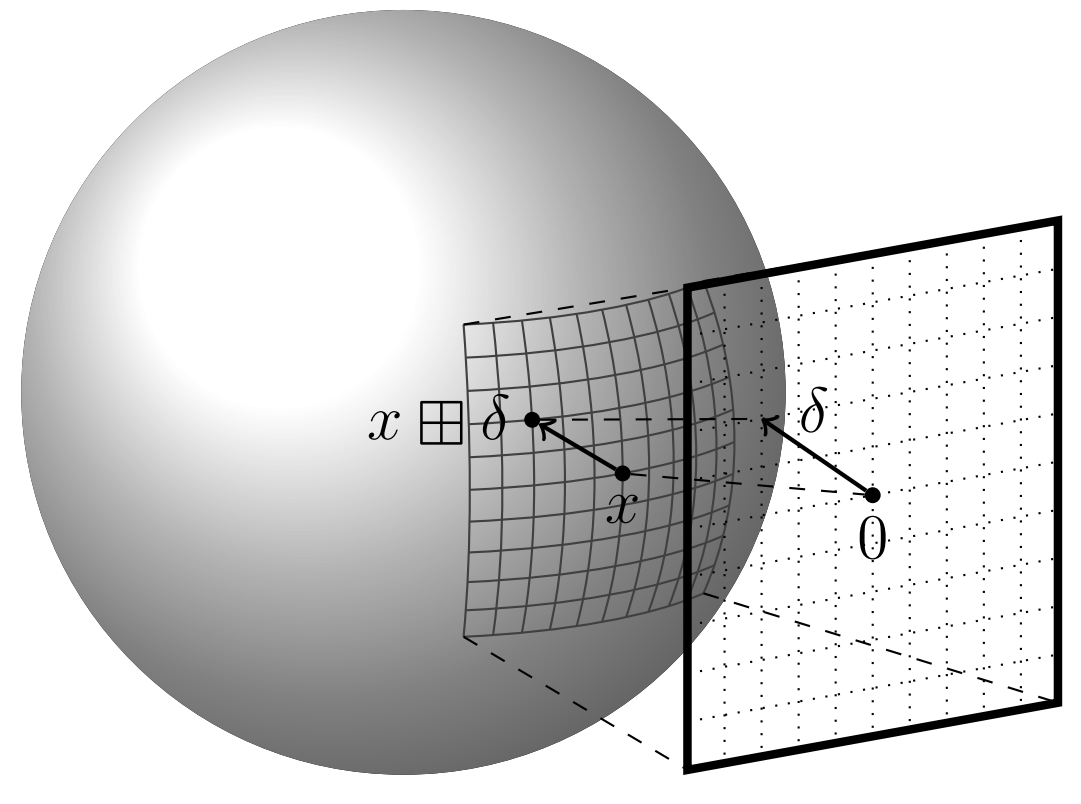
\includegraphics[width=0.7\linewidth]{Pictures/State_Estimation/Unscented_Kalman_Filter_on_Manifolds/Manifold_Mapping.png}
    \caption{Mapping a local neighborhood in the state space (here: on the unit sphere $\mathbb{S}^2$) into $\mathbb{R}^n$ (here: the plane) allows for the use of standard sensor fusion algorithms without explicitly encoding the global topological structure. Image and figure text taken from UKF-M paper.\textsuperscript{\cite{ukf_manifold}}}
    \label{fig:state-estimation-manifold-mapping}
\end{figure}
\noindent
To enable consistent state updates on a nonlinear manifold, the UKF-M introduces two generalized operators, $\boxplus$ and $\boxminus$, which replace standard addition and subtraction. They relate the manifold to its tangent space:
$$
\begin{aligned}
    \mathbf{x}' = \mathbf{x} \boxplus \boldsymbol{\delta} \\
    \boldsymbol{\delta} = \mathbf{y} \boxminus \mathbf{x}
\end{aligned}
$$
Note that $\boldsymbol{\delta}$ is \textit{not} the error state as used in the ESKF formulation. Instead, $\boldsymbol{\delta}$ represents a small perturbation defined in the local tangent space at $\mathbf{x}$, and can take any arbitrary value within that space.  
\\ \\
Here, $\mathbf{x}$ and $\mathbf{y}$ are elements on the manifold $\mathcal{M}$, while $\boldsymbol{\delta} \in T_\mathbf{x}\mathcal{M}$ is the corresponding vector in the tangent space. The $\boxplus$ operator applies a perturbation from the tangent space to move the state along the manifold, producing an updated manifold element $\mathbf{x}'$. Conversely, the $\boxminus$ operator computes the minimal difference between two manifold states by mapping that displacement back into the tangent space.  
\\ \\
Together, these two operators define a consistent way to move back and forth between the manifold $\mathcal{M}$ and its tangent space $T_\mathbf{x}\mathcal{M}$, enabling the UKF-M to perform all statistical operations (eks, mean and covariance propagation) in a locally Euclidean space while keeping the final state representation on the true manifold. 
\\ \\
In Euclidean space, these operators reduce to standard vector addition and subtraction, i.e.
$\mathbf{x}' = \mathbf{x} \boxplus \boldsymbol{\delta} = \mathbf{x} + \boldsymbol{\delta}$ and $\boldsymbol{\delta} = \mathbf{y} \boxminus \mathbf{x} = \mathbf{y} - \mathbf{x}$. However, on curved manifolds like $\mathbb{S}^3$, directly adding vectors can move the state off the manifold, violating its geometric constraints. To address this, the $\boxplus$ and $\boxminus$ operators rely on the exponential and logarithmic maps that move between the manifold and its tangent space:
$$
\begin{aligned}
    \mathbf{x} \boxplus \mathbf{\delta} &= \exp(\mathbf{\delta}) \circ \mathbf{x} &\qquad (Tangent \rightarrow Manifold) \\
    \mathbf{y} \boxminus \mathbf{x} &= \log(\mathbf{y} \circ \mathbf{x}^{-1}) &\qquad (Tangent \leftarrow Manifold)
\end{aligned}
$$
where $\circ$ denotes the group composition operator. The exponential map projects a tangent space perturbation onto the manifold, while the logarithmic map computes the smallest displacement between two manifold elements within the tangent space.  
\\ \\
These mappings are directly analogous to the Lie group relations (See Equations \ref{eq:lie-groups-and-manifold-exponential}-\ref{eq:lie-groups-and-manifold-logarithmic} and Figure \ref{fig:system-modeling-so3-se3})
$$
\begin{aligned}
    R &= \exp(\boldsymbol{\omega}^\times) &\qquad (Tangent \rightarrow Manifold) \\
    \boldsymbol{\omega} &= \log(R) &\qquad (Tangent \leftarrow Manifold)
\end{aligned}
$$
which connect a rotation matrix $R \in SO(3)$ and its corresponding rotation vector $\boldsymbol{\omega} \in \mathbb{R}^3$. In the UKF-M framework, the same concept generalizes to full state vectors composed of multiple manifold and Euclidean components.



\subsubsection{Manifold Operators for the Process Model}
In the UKF-M framework, the process model defined in Equation \ref{eq:kinematics-motion-model} evolves the system state over time using inertial measurements. Since the state vector
$$
    \mathbf{x} =
    \begin{bmatrix}
        \mathbf{p}_{b/O}^{n} & \mathbf{v}_{b/O}^{n} & \mathbf{q} & \mathbf{a}_b & \mathbf{\omega}_b
    \end{bmatrix}^\top
$$
contains both Euclidean components $(\mathbf{p}, \mathbf{v}, \mathbf{a}_b, \mathbf{\omega}_b)$ and a manifold component $(\mathbf{q} \in \mathbb{S}^3)$, the standard addition and subtraction operations used in classical UKF cannot be directly applied. The attitude quaternion lies on the unit sphere $\mathbb{S}^3$, which is a nonlinear manifold, meaning that the linear operations used for Euclidean states are not globally valid.  
\\ \\
To handle this properly, the UKF-M defines two special manifold consistent operators, $\boxplus$ and $\boxminus$, that map between the nonlinear manifold and its local tangent space. These operators are used throughout the prediction and update stages whenever states or covariances are combined or compared.

\paragraph{$\boxplus$: Mapping a tangent space perturbation to the manifold} \mbox{}\\[0.5em] \noindent
The $\boxplus$ operator defines how a state on the manifold is updated using a perturbation vector $\boldsymbol{\xi}$ that lives in the tangent space. In this formulation, $\mathbf{x}$ represents the nominal state on the manifold, while $\boldsymbol{\xi}$ is a small local offset expressed in the linear tangent space around $\mathbf{x}$. The tangent space acts as a flat, Euclidean approximation of the manifold near the current mean, allowing linear algebra operations such as addition and covariance computation to be performed safely.
\\ \\
Taking an example of sigma point generation from the UKF-M algorithm discussed later down bellow takes form
$$
    \mathcal{X} = \mathbf{x} \boxplus \boldsymbol{\xi}
$$
where $\mathbf{x}$ is the current estimated state and $\boldsymbol{\xi}$ represents a small perturbation drawn from the covariance in tangent space. The vector $\boldsymbol{\xi}$ has the same structure as the state but replaces the quaternion with a 3D rotation vector. Explicitly,
$$
    \mathbf{x} =
    \begin{bmatrix}
        \mathbf{p}_{b/O}^{n} & \mathbf{v}_{b/O}^{n} & \mathbf{q} & \mathbf{a}_b & \mathbf{\omega}_b
    \end{bmatrix}^\top \quad
    \boldsymbol{\xi} =
    \begin{bmatrix}
        \boldsymbol{\xi}_{p} & \boldsymbol{\xi}_{v} & \boldsymbol{\xi}_{\theta} & \boldsymbol{\xi}_{a_b} & \boldsymbol{\xi}_{w_b}
    \end{bmatrix}^\top
$$
Here, the quaternion $\mathbf{q}$ is an element of the unit hypersphere $\mathbb{S}^3$, while the vector $\boldsymbol{\xi}_{\theta} \in \mathbb{R}^3$ is a tangent space representation of a small rotation around the mean orientation.
\\ \\
In tangent space, quaternions do not exist, only 3D rotation vectors do. The vector $\boldsymbol{\xi}_{\theta}$ simply points in the direction and magnitude of the local rotational perturbation, describing how the attitude should change infinitesimally around the current estimate.
\\ \\
When converting this local perturbation back to the manifold, the rotation vector must be mapped to a unit quaternion on $\mathbb{S}^3$. This is done through the exponential map, which transforms a small 3D vector into a valid quaternion rotation. The mapping is
$$
    \mathbf{q}_{\boldsymbol{\xi}_{\theta}} \triangleq 
    \mathrm{Exp}\left(\tfrac{1}{2}\boldsymbol{\xi}_{\theta}\right) =
    \begin{bmatrix}
        \cos\left(\tfrac{|\boldsymbol{\xi}_{\theta}|}{2}\right) \\
        \frac{\boldsymbol{\xi}_{\theta}}{|\boldsymbol{\xi}_{\theta}|}
        \sin\left(\tfrac{|\boldsymbol{\xi}_{\theta}|}{2}\right)
    \end{bmatrix}
$$
The division by two appears because quaternion rotations encode angles that are twice the corresponding rotation vector magnitude. Using this, the complete state perturbation becomes
$$
    \mathbf{x} \boxplus \boldsymbol{\xi} =
    \begin{bmatrix}
        \mathbf{p}_{b/O}^{n} + \boldsymbol{\xi}_{p} \\
        \mathbf{v}_{b/O}^{n} + \boldsymbol{\xi}_{v} \\
        \mathbf{q} \otimes \mathrm{Exp}\left(\tfrac{1}{2}\boldsymbol{\xi}_{\theta}\right) \\
        \mathbf{a}_b + \boldsymbol{\xi}_{a_b} \\
        \mathbf{\omega}_b + \boldsymbol{\xi}_{\omega_b}
    \end{bmatrix}
$$
The linear components like position, velocity, and biases are updated using simple vector addition, since they exist in Euclidean space. The quaternion, however, must be updated multiplicatively using the exponential map to remain on the manifold $\mathbb{S}^3$. This ensures that every sigma point maintains unit norm and represents a valid orientation.
\\ \\
In essence, $\boldsymbol{\xi}$ is never a physical state but a local linear displacement defined in the tangent space. It expresses how much the manifold state should move in each direction, including rotation, to represent local uncertainty. When mapped back through $\boxplus$, the translational components shift linearly, while the rotational component \textit{``bends''} along the hypersphere surface via the exponential map. This process allows the UKF-M to handle quaternions and other manifold states consistently, performing uncertainty propagation and updates in linear tangent space while always keeping the resulting states valid on their nonlinear manifold.

\paragraph{$\boxminus$: Mapping a manifold difference to the tangent space} \mbox{}\\[0.5em] \noindent
The $\boxminus$ operator defines how the difference between two states on the manifold, $\mathbf{x}_1$ and $\mathbf{x}_2$, is expressed as a perturbation vector in the tangent space. While $\boxplus$ projects a local perturbation from the tangent space onto the manifold, $\boxminus$ performs the inverse operation, it measures how far one manifold element is from another and maps that difference back into the linear tangent domain. This operation is essential for computing residuals, innovations, and covariance updates within the UKF-M, since all statistical quantities must reside in Euclidean tangent space.
\\ \\
For two states
$$
    \mathbf{x}_1 =
    \begin{bmatrix}
        \mathbf{p}_1 & \mathbf{v}_1 & \mathbf{q}_1 & \mathbf{b}_{a_1} & \mathbf{b}_{\omega_1}
    \end{bmatrix}^\top,
    \quad
    \mathbf{x}_2 =
    \begin{bmatrix}
        \mathbf{p}_2 & \mathbf{v}_2 & \mathbf{q}_2 & \mathbf{b}_{a_2} & \mathbf{b}_{\omega_2}
    \end{bmatrix}^\top
$$
the manifold consistent subtraction is defined as
$$
    \mathbf{x}_1 \boxminus \mathbf{x}_2 =
    \begin{bmatrix}
        \mathbf{p}_1 - \mathbf{p}_2 \\
        \mathbf{v}_1 - \mathbf{v}_2 \\
        2\,\mathrm{Log}\!\left(\mathbf{q}_2^{-1} \otimes \mathbf{q}_1\right) \\
        \mathbf{b}_{a_1} - \mathbf{b}_{a_2} \\
        \mathbf{b}_{\omega_1} - \mathbf{b}_{\omega_2}
    \end{bmatrix}
$$
Here, the linear quantities (position, velocity, and sensor biases) can be subtracted directly, as they live in Euclidean space. However, the quaternion part requires special handling because it resides on the unit hypersphere $\mathbb{S}^3$. To obtain a meaningful rotational difference between $\mathbf{q}_1$ and $\mathbf{q}_2$, the relative rotation
$$
    \mathbf{q}_{\text{relative}} = \mathbf{q}_2^{-1} \otimes \mathbf{q}_1
$$
is computed, representing the rotation that brings $\mathbf{q}_2$ to $\mathbf{q}_1$.
\\ \\
This relative quaternion is then converted into its corresponding tangent space vector using the logarithmic map, which projects the quaternion from $\mathbb{S}^3$ to $\mathbb{R}^3$. For a quaternion $\mathbf{q}_{\text{relative}} = [q_w, q_{\mathbf{v}}]^\top$ where $q_{\mathbf{v}} = [q_x, q_y, q_z]^T$ composed of scalar $q_w$ and vector $q_{\mathbf{v}}$ parts, the mapping is defined as
$$
    \boldsymbol{\theta}_{\text{relative}} \triangleq
    \mathrm{Log}(\mathbf{q}_{\text{relative}}) =
    \begin{cases}
        \displaystyle \frac{2 \, \arctan2(\|q_{\mathbf{v}}\|, q_w)}{\|q_{\mathbf{v}}\|}\,q_{\mathbf{v}}, & \text{if } \|q_{\mathbf{v}}\| \neq 0 \\[1em]
        \mathbf{0}, & \text{otherwise}
    \end{cases}
$$
The result of this operation is a 3D rotation vector $\boldsymbol{\theta}_{\text{relative}} \in \mathbb{R}^3$ that lies in the tangent space of the unit quaternion manifold. This vector points along the rotation axis and has a magnitude equal to the rotation angle between the two orientations. It therefore provides a minimal, linear representation of the orientation error. The factor of two ensures consistency with the quaternion exponential map used in the $\boxplus$ operator.
\\ \\
Intuitively, $\boxminus$ answers the question: “What small rotation and translation in tangent space would transform $\mathbf{x}_2$ into $\mathbf{x}_1$?” For Euclidean components, the answer is simply the difference between vectors. For rotational components, it is the smallest rotation vector on the manifold surface that aligns $\mathbf{q}_2$ with $\mathbf{q}_1$. By performing this mapping, the UKF-M can compute orientation residuals, innovations, and covariance deviations in a consistent, linearized space without ever violating the unit quaternion constraint.

\paragraph{Interpretation} \mbox{}\\[0.5em] \noindent
The $\boxplus$ and $\boxminus$ operators together define the mathematical bridge between the nonlinear manifold and its locally linear tangent space, ensuring that attitude, position, and bias states are updated consistently. The $\boxplus$ operator applies a perturbation from tangent space to the manifold, producing a new valid state on $\mathbb{S}^3$, while the $\boxminus$ operator performs the reverse, projecting the difference between two manifold states back into tangent space where linear operations such as mean and covariance can be computed.
\\ \\
Within the UKF-M process framework, $\boxplus$ is used when generating sigma points or updating the state estimate after correction, effectively moving the state along the manifold surface in response to perturbations. Conversely, $\boxminus$ is used when comparing predicted and updated states or computing innovations, allowing differences in orientation and position to be expressed in a linearized space suitable for statistical computation.
\\ \\
Together, these mappings preserve the unit quaternion constraint and maintain full geometric consistency of the nonlinear attitude dynamics described by the process model \ref{eq:kinematics-motion-model}, preventing normalization errors or distortion of uncertainty during repeated prediction and update cycles.



\subsubsection{Manifold Operators for the Measurement Model}
The measurement model in Equation \ref{eq:aiding-measurement-model} maps the nonlinear navigation state $\mathbf{x}$ into a measurable quantity $\mathbf{z}$ composed of GNSS position and yaw. The measurement manifold therefore combines both Euclidean and circular components:
$$
    \mathbf{z} =
    \begin{bmatrix}
        \mathbf{p}_{b/O}^{n} \\
        \psi
    \end{bmatrix},
    \quad
    \mathbf{z} \in \mathbb{R}^3 \times \mathbb{S}^1
$$
where $\psi$ is the yaw angle, living on the circle manifold $\mathbb{S}^1$. 
\\ \\
The process $f(\cdot)$ and measurement $h(\cdot)$ manifolds thus differ in structure, while the state includes quaternion orientation $\mathbf{q} \in \mathbb{S}^3$, the measurement only includes a single angular degree of freedom (yaw) and the position.  

\paragraph{$\boxplus$: Mapping a tangent space perturbation to the manifold} \mbox{}\\[0.5em] \noindent
The measurement residual must be computed in the tangent space of the measurement manifold. This ensures that angular differences are represented as the shortest signed distance on the circle, avoiding discontinuities around $\pm\pi$. 
\\ \\ 
Given an actual measurement $\mathbf{z}$ and predicted measurement $\hat{\mathbf{z}} = h(\hat{\mathbf{x}})$, the innovation is
$$
    \boldsymbol{\nu} = \mathbf{z} \boxminus \hat{\mathbf{z}} =
    \begin{bmatrix}
        \mathbf{z}_p - \hat{\mathbf{z}}_p \\
        \mathrm{wrap\_to\_pi}(\mathbf{z}_\psi - \hat{\mathbf{z}}_\psi)
    \end{bmatrix}
$$
The function $\mathrm{wrap\_to\_pi}(\cdot)$ ensures that angular differences are represented within the principal interval $[-\pi, \pi]$, preventing discontinuities when the heading crosses the $\pm\pi$ boundary. In practice, this operation computes the smallest signed angular distance between the measured and predicted yaw angles. Without this normalization, an orientation difference between $179^\circ$ and $-179^\circ$ would be interpreted as a large $358^\circ$ error, even though the true discrepancy is only $2^\circ$. By wrapping the result, the innovation $\boldsymbol{\nu}$ remains continuous and physically meaningful across the entire rotation range, ensuring numerical stability and consistency in the filter update. The resulting innovation vector thus lies in the tangent space $\mathbb{R}^3 \times \mathbb{R}$, allowing it to be used directly in the covariance update and gain computation.

\paragraph{$\boxminus$: Mapping a manifold difference to the tangent space} \mbox{}\\[0.5em] \noindent
In certain filtering frameworks (such as smoothing or iterative measurement correction), a $\boxplus$ operation may be required to reapply a correction in measurement space. For example, if the predicted measurement $\hat{\mathbf{z}}$ must be adjusted by a correction $\delta\mathbf{z}$, the operation is defined as
$$
    \hat{\mathbf{z}} \boxplus \delta\mathbf{z} =
    \begin{bmatrix}
        \hat{\mathbf{z}}_p + \delta\mathbf{z}_p \\
        \mathrm{wrap\_to\_pi}(\hat{\mathbf{z}}_\psi + \delta\mathbf{z}_\psi)
    \end{bmatrix}
$$
ensuring that angular corrections respect the periodic geometry of $\mathbb{S}^1$.  

\paragraph{Interpretation} \mbox{}\\[0.5em] \noindent
In the measurement model, the roles of $\boxplus$ and $\boxminus$ differ from those in the process model. The $\boxminus$ operator is the one predominantly used, as it computes the innovation between the actual and predicted measurements in a geometrically consistent way. This operation ensures that the angular residuals, such as yaw differences, are always represented as the smallest signed angle, maintaining continuity across the $\pm\pi$ boundary.  
\\ \\
The $\boxplus$ operator, although formally defined for completeness, is rarely used in practical state estimation filters such as the UKF-M. It becomes relevant only in specific cases, such as iterative measurement refinement or optimization based frameworks, where perturbations in measurement space must be mapped back onto the manifold.  
\\ \\
Together, these operators maintain the consistency between the nonlinear measurement manifold $\mathbb{R}^3 \times \mathbb{S}^1$ and its tangent space. The $\boxminus$ operator enables proper innovation computation for covariance updates, while $\boxplus$ ensures that potential corrections respect the manifold geometry. This separation guarantees that both position and angular measurements are handled accurately within their respective geometric domains, preserving filter stability and correctness.



\subsubsection{MeanOfSigmaPoints() on Manifolds}
When sigma points lie on a manifold, their average cannot be computed using standard Euclidean addition. Unlike vector spaces, manifolds do not support global linear operations such as direct addition or subtraction. Therefore, the mean must be defined geometrically as the point that minimizes the total squared distance to all sigma points when those distances are measured in the local tangent space. Formally, the mean $\mu$ is given by
$$
    \mu = \operatorname*{argmin}_{\mathbf{x}} 
    \sum_{i=0}^{2L} \| \mathcal{X}_i \boxminus \mathbf{x} \|^2
$$
This expression defines the manifold mean as the point that minimizes the weighted sum of squared tangent space distances between each sigma point $\mathcal{X}_i$ and the candidate mean $\mathbf{x}$. The $\boxminus$ operator computes the local difference between two manifold elements and maps that difference back into the tangent space, where distances are represented as standard Euclidean vectors.  
\\ \\
Intuitively, this means that rather than directly averaging points on the manifold, which would produce a result that leaves the manifold surface, the mean is found through a search process that balances all sigma points in the tangent space. The final $\mu$ lies on the manifold and represents the most symmetric and geometrically correct center of the sigma point cloud.  
\\ \\
To compute this mean in practice, we use an iterative fixed point algorithm:
\begin{equation}
    \begin{aligned}
        \mu_0 &= \mathcal{X}_0 \\
        \mu_{k+1} &= \mu_k \boxplus 
        \left( 
            \frac{1}{2L + 1} \, \sum_{i=0}^{2L} (\mathcal{X}_i \boxminus \mu_k)
        \right) \\
        \mu &= \lim_{k \to \infty} \mu_k
    \end{aligned}
\end{equation}
This iterative method refines an initial estimate $\mu_0$ (often chosen as the first sigma point or previous state estimate) until the mean converges to a point around which all sigma points are symmetrically distributed in the tangent space. Each iteration alternates between mapping manifold elements to the tangent space with $\boxminus$ and updating the mean on the manifold with $\boxplus$. The result is a process that moves back and forth between the curved manifold and its locally linear tangent space until equilibrium is reached.  
\\ \\
The first operation, $(\mathcal{X}_i \boxminus \mu_k)$, measures how far each sigma point $\mathcal{X}_i$ lies from the current mean estimate $\mu_k$ along the manifold. Since subtraction is undefined on a curved surface, $\boxminus$ projects this geometric difference into the tangent space at $\mu_k$, producing small linear displacement vectors that can be averaged safely. The average of these displacements,
$$
    \frac{1}{2L + 1} \, \sum_{i=0}^{2L} (\mathcal{X}_i \boxminus \mu_k)
$$
represents the average direction and magnitude by which the current mean estimate $\mu_k$ is offset from the true geometric center of the sigma points.  
\\ \\
It is important to note that in this formulation, the explicit sigma point weights $W_i^m$ and $W_i^c$ that appear in the classical UKF are no longer required. The UKF-M relies instead on the geometric symmetry of the sigma point distribution, where each positive perturbation has an equal negative counterpart. Because the sigma points are generated symmetrically around the mean using $\pm\sqrt{P}$, their contribution to the average naturally balances out. This symmetry ensures that the mean and covariance reconstruction are unbiased without needing explicit weighting factors. The normalization factor $\frac{1}{2L+1}$ simply ensures equal contribution from all points, maintaining the geometric consistency of the averaging process. In other words, this method depends purely on the manifolds local geometry rather than statistical weights designed for Euclidean Gaussian moments.  
\\ \\
If the averaged deviation in the tangent space is zero, it means that all sigma points are symmetrically arranged around $\mu_k$, and the iteration has converged. If not, the mean must be corrected. The update step is carried out using the $\boxplus$ operator,
$$
    \mu_{k+1} = \mu_k \boxplus \Delta\mu,
    \quad \text{where} \quad 
    \Delta\mu = \frac{1}{2L + 1} \, \sum_{i=0}^{2L} (\mathcal{X}_i \boxminus \mu_k)
$$
Here, $\Delta\mu$ is a small vector in the tangent space describing how to shift the current mean estimate toward the geometric center of the sigma points. The $\boxplus$ operator then maps this small correction vector from the tangent space back onto the manifold, updating $\mu_k$ into a new manifold element $\mu_{k+1}$. Each iteration therefore involves two transformations:  
\begin{enumerate}
    \item $\boxminus$: Tangent $\leftarrow$ Manifold, then measure displacements in a linear domain.
    \item $\boxplus$: Tangent $\rightarrow$ Manifold, then update the mean in the curved domain.
\end{enumerate}
Repeating this process ensures that the mean estimate remains on the manifold at every step while progressively converging toward the true center in tangent space terms. The algorithm stops once the magnitude of the correction vector becomes sufficiently small:
$$
    \|\Delta\mu\| = \left\| \frac{1}{2L + 1} \, \sum_{i=0}^{2L} (\mathcal{X}_i \boxminus \mu_k) \right\|
$$
When $\|\Delta\mu\|$ drops below a user defined tolerance $\epsilon$ (typically $10^{-6}$ or $10^{-8}$), the iteration is terminated:
$$
    \text{stop if } \|\Delta\mu\| < \epsilon
$$
This convergence criterion ensures that further updates would no longer produce meaningful changes, meaning the mean has stabilized.  
\\ \\
Conceptually, this iterative mean calculation behaves like computing an expected value, but in a manifold consistent manner. Instead of adding the sigma points directly, which would violate manifold geometry, the algorithm repeatedly measures deviations in tangent space, computes an average there, and re-projects the correction back to the manifold using $\boxplus$. Through successive iterations, the mean converges to the point that minimizes the sum of squared tangent space residuals to all sigma points. The final $\mu$ lies exactly on the manifold, is geometrically correct, and provides the proper reference for subsequent covariance computation.  
\\ \\
This entire operation is conveniently encapsulated by the function call
$$
    \mu = \text{MeanOfSigmaPoints}(\mathcal{X}_i)
$$
which internally performs the iterative procedure described above, providing a consistent and geometrically valid manifold mean.



\subsubsection{Filter Algorithm: Prediction Step}
In the Unscented Kalman Filter on Manifolds (UKF-M), the propagation follows the same general structure as the classical Unscented Kalman Filter but introduces one essential geometric correction. In the UKF-M, all statistical operations such as averaging, difference calculation, and covariance computation are performed in the tangent space of the manifold rather than directly on the manifold itself. The reason is that linear algebra operations such as addition or subtraction are only defined in Euclidean vector spaces, while a manifold is curved and does not support these operations globally.  
\\ \\
The tangent space is a locally flat linear approximation of the manifold that touches it at the current state estimate $\hat{\mathbf{x}}$. Inside this tangent space, we can safely perform vector operations and treat perturbations as if the system were linear, while on the manifold itself, only composition and mapping operations are valid. This separation is the key idea of the UKF-M, where the state lives on the manifold, but the uncertainty around that state, represented by the covariance matrix $P$, lives in the tangent space.  
\\ \\
An important difference from the standard UKF is that in the UKF-M, no explicit sigma point weights $W_i^m$ or $W_i^c$ are used during the mean and covariance computations. Instead, the algorithm relies purely on the geometric symmetry of the sigma point distribution. In the classical UKF, the weights are necessary because the sigma points are designed to reproduce the exact first and second moments of a Gaussian distribution in Euclidean space, which requires careful weighting. However, in the UKF-M, the sigma points are constructed symmetrically around the mean in the tangent space, and this symmetry ensures that the unweighted average of their spread already provides a correct and unbiased representation of the local uncertainty. Each positive perturbation has a corresponding negative one, canceling any bias in the mean and producing a covariance that correctly represents the local shape of the uncertainty region. This geometric symmetry removes the need for explicit weighting and simplifies both the mean and covariance reconstruction.  
\\ \\
The propagation begins by generating these symmetric sigma points in the tangent space around the current mean $\hat{\mathbf{x}}$,  
\begin{equation}
    \begin{aligned}
        \boldsymbol{\xi}_0 &= \mathbf{0} \\
        \boldsymbol{\xi}_i &= \sqrt{P_i}              && i = 1, \ldots, L \\
        \boldsymbol{\xi}_i &= -\sqrt{P_{i - L}}       && i = L+1, \ldots, 2L
    \end{aligned}
\end{equation}
Each $\boldsymbol{\xi}_i$ is a perturbation vector that expresses a small local offset in the tangent space, describing how the true state might deviate from the mean. The scaling factor is absorbed into the square root, and all sigma points are equally important due to their symmetric layout.  
\\ \\
Because the process model $f_d(\cdot)$ is defined directly on the manifold, these perturbations cannot be used as-is. They must first be mapped to actual states on the manifold. This is done using the $\boxplus$ operator,  
$$
    \mathcal{X}_i = \hat{\mathbf{x}} \boxplus \boldsymbol{\xi}_i
$$
The $\boxplus$ operator takes the current state $\hat{\mathbf{x}}$ on the manifold and a tangent vector $\boldsymbol{\xi}_i$ in its local tangent space and produces a new manifold element. It effectively “moves” the state along the manifold surface in the direction described by $\boldsymbol{\xi}_i$. This step ensures that all sigma points $\mathcal{X}_i$ are valid manifold elements, such as normalized quaternions or valid pose transformations.  
\\ \\
Each of these manifold sigma points is then propagated through the nonlinear discrete dynamics model,  
$$
    \mathcal{X}_i^- = f_d(\mathcal{X}_i, \mathbf{u})
$$
After propagation, all $\mathcal{X}_i^-$ remain on the manifold because $f_d(\cdot)$ defines evolution rules that preserve the manifold structure. For example, quaternion propagation keeps unit norm, and rigid-body motion remains on $\mathrm{SE}(3)$.  
\\ \\
The next step is to determine the predicted mean state $\hat{\mathbf{x}}^-$. Since the propagated sigma points $\mathcal{X}_i^-$ now lie on the manifold, their mean must also lie on the same manifold. Because manifolds do not support standard addition or averaging, the mean cannot be computed as a simple arithmetic sum. Instead, we define a dedicated function that estimates the manifold mean of a set of sigma points,  
$$
    \hat{\mathbf{x}}^- = \text{MeanOfSigmaPoints}(\mathcal{X}_i^-)
$$
This function represents a general procedure that finds the best mean state on the manifold based on the geometry of the sigma points. Internally, it performs the necessary manifold-consistent averaging using the $\boxminus$ operation to measure distances in the tangent space, returning a valid and accurate mean estimate. The resulting $\hat{\mathbf{x}}^-$ lies on the manifold and becomes the new predicted state mean.
\\ \\
Once the mean is found, we must express the uncertainty of the state distribution around this mean. This cannot be done directly on the manifold because addition and subtraction between manifold elements are not globally valid. Therefore, all propagated sigma points $\mathcal{X}_i^-$ are mapped back into the tangent space centered at $\hat{\mathbf{x}}^-$ using the $\boxminus$ operator,  
$$
    \boldsymbol{\xi}_i^- = \mathcal{X}_i^- \boxminus \hat{\mathbf{x}}^-
$$
This step is crucial because the covariance $P$ represents uncertainty in a linear space. It encodes how much the state may vary locally around the mean. If we attempted to compute $P$ directly on the manifold, we would violate its geometry, as covariance addition and subtraction would move the result off the manifold. By using the $\boxminus$ operator, each sigma point is projected back into the tangent space, effectively flattening the curved neighborhood around $\hat{\mathbf{x}}^-$ into a locally linear space where covariance computation is valid.  
\\ \\
The predicted covariance is then reconstructed from these tangent space deviations using an unweighted symmetric formulation,
$$
    P^- = \frac{1}{2}\sum_{i=1}^{2L} \boldsymbol{\xi}_i^- (\boldsymbol{\xi}_i^-)^\top + Q
$$
Here, $P^-$ represents the predicted covariance of the state in the tangent space, while the mean $\hat{\mathbf{x}}^-$ remains strictly on the manifold. The covariance $P^-$ captures the spread and orientation of uncertainty in local linear coordinates, effectively describing how much and in which directions the state can vary around the mean within the manifolds neighborhood.  
\\ \\
In this formulation, explicit weighting coefficients such as $W_i^m$ or $W_i^c$, which are typically used in the classical UKF are no longer present. The reason is that in the UKF-M, sigma points are generated in a geometrically symmetric way around the mean, using $\pm\sqrt{P}$. This symmetric structure inherently guarantees that the contributions from all sigma points are balanced and unbiased. Each positive perturbation has an equal and opposite negative counterpart, ensuring that the overall distribution remains centered around zero in the tangent space. As a result, the average and covariance of these symmetric deviations can be computed without statistical weighting because the geometry itself enforces equilibrium.  
\\ \\
In contrast, the traditional UKF relies on asymmetric scaling and weighting to preserve the exact first and second statistical moments of a Gaussian distribution in Euclidean space. Those weights compensate for the uneven influence of the central sigma point and its surrounding samples. However, on a manifold, this probabilistic interpretation is less meaningful since addition and subtraction are not globally defined. The UKF-M instead treats the sigma points as a symmetric geometric sampling of local uncertainty rather than as discrete weighted samples of a probability distribution. Consequently, the covariance is reconstructed purely from geometry, using uniform contributions from each tangent space deviation. The factor $\frac{1}{2}$ in the equation serves as a normalization constant that reflects the fact that each dimension contributes both a positive and a negative sigma point of equal magnitude.  
\\ \\
This geometric treatment greatly simplifies the covariance reconstruction and ensures that the resulting $P^-$ is always consistent with the local curvature of the manifold. The tangent-space deviations $\boldsymbol{\xi}_i^-$ provide valid Euclidean displacement vectors that can be combined using standard linear algebra, while the mean $\hat{\mathbf{x}}^-$ remains on the nonlinear manifold surface. In this way, the UKF-M cleanly separates the roles of geometry and statistics: $\hat{\mathbf{x}}^-$ captures the nonlinear evolution of the state itself, and $P^-$ describes the uncertainty in a locally flat, linearized representation.  
\\ \\
This separation between the manifold domain for the state and the tangent-space domain for the covariance is fundamental to the design of manifold-based filters. The $\boxplus$ operator maps tangent perturbations onto the manifold to form valid states, while the $\boxminus$ operator maps manifold differences back into the tangent space for linear operations. These two operators together maintain full geometric consistency throughout the propagation process. Without this dual-space treatment, adding or subtracting states directly would produce inconsistencies—potentially leading to drift, loss of normalization, or distorted covariance when operating in curved spaces such as rotations or poses.  
\\ \\
Therefore, in the UKF-M, the covariance reconstruction step is not just a numerical simplification but a direct consequence of respecting the manifold geometry. By leveraging the symmetry of the sigma point distribution, the filter avoids the need for weighting coefficients, preserves local geometric balance, and keeps the statistical representation consistent with the curvature of the underlying manifold. The state mean $\hat{\mathbf{x}}$ always resides on the manifold, while the covariance $P$ always resides in its tangent space, ensuring that both the geometry and uncertainty of the system are correctly and consistently represented throughout propagation.



\subsubsection{Filter Algorithm: Correction Step}
After the propagation step, the Unscented Kalman Filter on Manifolds (UKF-M) incorporates new sensor information to refine the predicted state estimate. The goal of the update stage is to compare the predicted measurement with the actual sensor measurement and then correct the state estimate in a way that is consistent with the manifold geometry.  
\\ \\
The overall process closely mirrors the classical UKF, but all operations that involve addition or subtraction of states or measurements must be performed in the corresponding tangent spaces. The reason is the same as before: the state $\hat{\mathbf{x}}$ lives on a nonlinear manifold, while both measurement innovations and covariance updates are linear statistical quantities that can only exist in Euclidean vector spaces. Therefore, throughout the update step, the UKF-M repeatedly moves between the manifold and its tangent space using the $\boxplus$ and $\boxminus$ operators.  
\\ \\
The update begins with the predicted state mean $\hat{\mathbf{x}}^-$ and covariance $P^-$. Using these, a new set of sigma points is generated in the tangent space centered at $\hat{\mathbf{x}}^-$,  
\begin{equation}
    \begin{aligned}
        \boldsymbol{\xi}_0 &= \mathbf{0} \\
        \boldsymbol{\xi}_i &= \sqrt{P_i^-}              && i = 1, \ldots, L \\
        \boldsymbol{\xi}_i &= -\sqrt{P_{i - L}^-}       && i = L+1, \ldots, 2L
    \end{aligned}
\end{equation}
Each $\boldsymbol{\xi}_i$ again represents a small perturbation in the tangent space, describing local uncertainty around the current mean. These perturbations are mapped back onto the manifold to form actual state sigma points,  
$$
    \mathcal{X}_i^- = \hat{\mathbf{x}}^- \boxplus \boldsymbol{\xi}_i
$$
Each $\mathcal{X}_i^-$ now represents a valid manifold state, for instance, a quaternion with unit norm or a valid pose transformation in $\mathrm{SE}(3)$.  
\\ \\
Each of these manifold sigma points is then passed through the nonlinear measurement model $h(\cdot)$,  
$$
    \mathcal{Z}_i = h(\mathcal{X}_i^-)
$$
which predicts what the measurement would look like for each sigma point. The resulting set of $\mathcal{Z}_i$ points represents a distribution of predicted measurements in the measurement space. Depending on the sensor, this space can itself be Euclidean (for example GNSS position) or also contain manifold elements (for example, angles on $\mathbb{S}^1$ or quaternions on $\mathbb{S}^3$).  
\\ \\
The predicted measurement mean $\hat{\mathbf{z}}$ is then computed. Since the measurement space may also include manifold valued quantities, such as orientations or angular variables, a direct arithmetic average is not valid. Instead, use the same consistent geometric averaging operation as for the state mean. The mean of the predicted measurement sigma points is obtained using the function
$$
    \hat{\mathbf{z}} = \text{MeanOfSigmaPoints}(\mathcal{Z}_i)
$$
This function performs manifold consistent averaging of all predicted measurement sigma points $\mathcal{Z}_i$ around an initial estimate $\hat{\mathbf{z}}$. It iteratively maps the sigma points into the tangent space using $\boxminus$, computes their weighted average deviation, and updates the mean on the manifold with $\boxplus$ until convergence. The resulting $\hat{\mathbf{z}}$ lies exactly on the measurement manifold, representing the central point where the sigma points are symmetrically distributed in the tangent space sense, ensuring a geometrically valid and consistent measurement mean.
\\ \\
Once the mean $\hat{\mathbf{z}}$ is obtained, all predicted measurement sigma points are mapped back into the tangent space at $\hat{\mathbf{z}}$ using the $\boxminus$ operator,  
$$
    \boldsymbol{\zeta}_i = \mathcal{Z}_i \boxminus \hat{\mathbf{z}}
$$
These tangent-space deviations $\boldsymbol{\zeta}_i$ describe how the predicted measurements vary locally around their mean in a linear space, which is necessary for computing covariances. Using these deviations, the measurement innovation covariance is calculated as,  
$$
    S = \frac{1}{2} \sum_{i=0}^{2L} \boldsymbol{\zeta}_i \boldsymbol{\zeta}_i^\top + R
$$
where $R$ is the measurement noise covariance matrix. The matrix $S$ thus represents the total uncertainty in the predicted measurement, combining both the propagated state uncertainty and the sensor noise.  
\\ \\
Next, the cross-covariance between the state and the measurement is computed. To do this consistently, we express both quantities in their respective tangent spaces. The state deviations are given by $\boldsymbol{\xi}_i^- = \mathcal{X}_i^- \boxminus \hat{\mathbf{x}}^-$, and the measurement deviations are the previously computed $\boldsymbol{\zeta}_i = \mathcal{Z}_i \boxminus \hat{\mathbf{z}}$. The cross-covariance is therefore,  
$$
    P_{xz} = \frac{1}{2} \sum_{i=0}^{2L} \boldsymbol{\xi}_i^- \boldsymbol{\zeta}_i^\top
$$
This matrix expresses how variations in the state tangent space correspond to variations in the predicted measurement tangent space, effectively linking the two spaces through their local linear approximations.  
\\ \\
The Kalman gain is now obtained as,  
$$
    K = P_{xz} S^{-1}
$$
which defines how much the state estimate should be corrected based on the measurement innovation.  
\\ \\
The innovation itself is computed as the difference between the actual measurement $\mathbf{z}$ and the predicted mean $\hat{\mathbf{z}}$,  
$$
    \boldsymbol{\nu} = \mathbf{z} \boxminus \hat{\mathbf{z}}
$$
Note that this operation also uses the manifold-aware subtraction, because the measurement may include angular or orientation components. The innovation vector $\boldsymbol{\nu}$ thus lives in the tangent space of the measurement manifold.  
\\ \\
After computing the Kalman gain, the correction step refines the predicted mean and covariance based on the new measurement.  
\\ \\  
The first step is to compute the correction vector in the tangent space of the state manifold,
$$
    \boldsymbol{\delta} = K \boldsymbol{\nu}
$$
This vector represents the optimal adjustment of the predicted state in the local tangent space.  
The updated uncertainty of this correction is obtained as
$$
    P' = P^- - K S K^\top
$$
which represents the new covariance of the correction vector $\boldsymbol{\delta}$ after the measurement information has been incorporated.
\\ \\
Using $\boldsymbol{\delta}$ and $P'$, a new set of sigma points is created to represent the corrected uncertainty around the predicted mean.  
In the tangent space, the sigma points are defined as
\begin{equation}
    \begin{aligned}
        \boldsymbol{\xi}'_0 &= \boldsymbol{\delta} \\
        \boldsymbol{\xi}'_i &= \boldsymbol{\delta} + \sqrt{P_i^-}              && i = 1, \ldots, L \\
        \boldsymbol{\xi}'_i &= \boldsymbol{\delta} - \sqrt{P_{i - L}^-}       && i = L+1, \ldots, 2L
    \end{aligned}
\end{equation}
These sigma points capture the spread of the post update uncertainty in the tangent space.  
\\ \\
Each tangent space sigma point is then mapped back onto the manifold around the predicted mean using the $\boxplus$ operator,
$$
    \mathcal{X}'_i = \hat{\mathbf{x}}^- \boxplus \boldsymbol{\xi}'_i
$$
This produces a new set of manifold sigma points $\mathcal{X}'_i$ that describe the updated state distribution after the measurement correction.  
\\ \\
The corrected state mean is then obtained by computing the manifold consistent average of these sigma points,
$$
    \hat{\mathbf{x}}^+ = \text{MeanOfSigmaPoints}(\mathcal{X}'_i)
$$
This operation finds the manifold point that minimizes the weighted squared tangent-space distances to all sigma points, ensuring that $\hat{\mathbf{x}}^+$ lies exactly on the manifold and represents the most likely corrected state.  
\\ \\
Finally, the updated covariance is computed from the spread of the new sigma points around the corrected mean in the tangent space,
$$
    P^+ = \frac{1}{2}\sum_{i=0}^{2L}
    [\,\mathcal{X}'_i \boxminus \hat{\mathbf{x}}^+\,]
    [\,\mathcal{X}'_i \boxminus \hat{\mathbf{x}}^+\,]^\top
$$
This final covariance $P^+$ captures the remaining uncertainty in the tangent space centered at $\hat{\mathbf{x}}^+$ and ensures full geometric consistency between the state and its uncertainty.
\\ \\
For systems that include quaternions or other unit-norm quantities, it is common to re-normalize the quaternion after the update step to correct for small numerical drift,  
$$
    \mathbf{q}^+ \leftarrow \frac{\mathbf{q}^+}{\|\mathbf{q}^+\|}
$$
This normalization step ensures that orientation remains physically valid and consistent with the manifold structure.  
\\ \\
In summary, the update step of the UKF-M carefully keeps the separation between the manifold and its tangent spaces. The state mean $\hat{\mathbf{x}}$ always remains on the manifold, while the covariance $P$ and all perturbations live in the tangent space. The $\boxplus$ operator moves perturbations from tangent to manifold, while $\boxminus$ maps differences from manifold back to tangent. This bidirectional mapping ensures that the state update remains geometrically consistent while allowing covariance and innovation computations to be performed in a locally linear space. The mean recomputation for both $\hat{\mathbf{z}}$ and $\hat{\mathbf{x}}^+$ follows the same principle as before: they are defined as the manifold elements minimizing the weighted residuals of their sigma points in their respective tangent spaces. Through these mappings, the UKF-M performs a statistically correct and geometrically sound measurement correction step, preserving both the nonlinear geometry and the probabilistic consistency of the filter.



\subsubsection{Advantages and Practical Aspects}
UKF-M provides several key advantages over traditional linearization based filters such as EKF and ESKF. Unlike these approaches, UKF-M does not rely on Jacobians, thereby eliminating the need for analytical derivations, symbolic differentiation, and the discretization errors that often occur in complex nonlinear systems. This not only simplifies implementation but also removes a common source of modeling mistakes. Furthermore, the UKF-M preserves full 2nd order accuracy during nonlinear mean and covariance propagation, resulting in more consistent and stable estimates in systems with strong non-linearities.  
\\ \\
Because the filter operates directly on manifolds, it naturally supports state representations that live in non Euclidean spaces such as rotation groups $\mathrm{SO}(3)$, unit quaternions $\mathbb{S}^3$, and rigid body poses $\mathrm{SE}(3)$. This allows seamless integration of mixed state variables like positions, velocities, orientations, and sensor biases within a single unified framework. Orientation handling is intrinsically consistent, avoiding the small angle approximations often required in EKF and ESKF formulations. The manifold formulation also removes the need for tuning heuristic scaling parameters such as $\alpha$, $\beta$, and $\kappa$, which in the classical UKF can significantly affect numerical stability and convergence. By relying purely on symmetric sigma point geometry, the UKF-M achieves a robust representation of uncertainty on curved spaces.  
\\ \\
Compared to the standard UKF, the manifold formulation is more general and geometrically consistent. It can be applied to arbitrary state spaces, including Lie groups and hybrid Euclidean manifold models, without modification. This generality makes the UKF-M particularly powerful in robotics and navigation, where states often include rotations, orientations, or transformations that cannot be treated with standard linear algebra.  
\\ \\
The main trade off of the UKF-M lies in computational cost. While it avoids the analytical burden of Jacobians, it replaces it with additional numerical computation. Each propagation and update step requires evaluating the nonlinear dynamics and measurement models for multiple sigma points, as well as performing iterative manifold averaging to compute the new mean. This sample based approach demands more processing than linearized filters, but modern hardware can easily accommodate it. Thus, while mathematically heavier, UKF-M is often simpler and more maintainable from a programming perspective, since all model functions can be implemented directly without differentiation.  
\\ \\
In applications such as SLAM and inertial navigation, this balance of simplicity, robustness, and geometric correctness makes the UKF-M a preferred choice. It provides accurate estimation of both position and orientation without relying on Jacobians or linearization, offering similar or superior accuracy to ESKF while being easier to maintain and extend. Although the increased computational demand can be a limitation for resource constrained systems, it is negligible for modern embedded platforms equipped with SBC. In the context of this thesis, the microAmpere ASV provides sufficient processing power, meaning that computation and memory are not bottlenecks for state estimation. Instead, the primary computational challenge lies in managing and optimizing the ever expanding SLAM map, not in running the filter itself.  
\\ \\
For these reasons, the UKF-M is adopted in this work as the primary state estimation framework. It offers a strong combination of theoretical rigor, implementation simplicity, and robust performance in nonlinear and manifold constrained systems, making it ideal for the requirements of marine autonomy, SLAM, and inertial navigation on the microAmpere ASV.
